% !TEX encoding = UTF-8 Unicode
% !TEX spellcheck = en-US


% This is the root file of your thesis: thesis.tex
% A line starting with % is a comment. In some cases, I have included a command preceded by a %. You may activate the command by removing the %.

%%===================================
\documentclass[12pt]{report}
\usepackage{ramsstyle}
%%===================================
%Write the various parts of your thesis as separate files and include them into the main file by the command \include{name of included file}. When you compile the LaTeX file, you may choose which subfiles to include by the command

%\includeonly{chapter01,chapter02}

%%===================================
\begin{document}
% !TEX encoding = UTF-8 Unicode
%!TEX root = thesis.tex
% !TEX spellcheck = en-US

%This is the Titlepage
%%=========================================
\thispagestyle{empty}
\mbox{}\\[6pc]
\begin{center}
\Huge{Web and Social Media Security}\\[2pc]

\Large{Emil Volckmar Ry, Jan Lindemann, Fabian Franz, \\ Audun Kjeldaas, Jørgen Ellingsen}\\[1pc]
\large{Desember 2016}\\[2pc]

PROJECT\\
Faculty of Informatics and Media Technology \\
Norwegian University of Science and Technology
\end{center}
\vfill

\noindent Supervisor: Prof. Dr. Bernhard M. Hämmerli

 % This is the titlepage
\setcounter{page}{0}
\pagenumbering{roman}
% !TEX encoding = UTF-8 Unicode
%!TEX root = thesis.tex
% !TEX spellcheck = en-US
%%=========================================
\addcontentsline{toc}{section}{Preface}
\section*{Preface}
Here, you give a brief introduction to your work. What it is (e.g., a Master's thesis in RAMS at NTNU as part of the study program xxx and\ldots), when it was carried out (e.g., during the autumn semester of 2021). If the project has been carried out for a company, you should mention this and also describe the cooperation with the company. You may also describe how the idea to the project was brought up.

You should also specify the assumed background of the readers of this report (who are you writing for).\\[2cm]

\begin{center}
Gj{\o}vik, Desember 2016\\[1pc]
Jørgen Ellingsen
\end{center}
% !TEX encoding = UTF-8 Unicode
%!TEX root = thesis.tex
% !TEX spellcheck = en-US
%%=========================================
\addcontentsline{toc}{section}{Acknowledgment}
\section*{Acknowledgment}
I would like to thank the following persons for their great help during \ldots

If the project has been carried out in cooperation with an external partner (e.g., a company), you should acknowledge the contribution and give thanks to the involved persons.

You should also acknowledge the contributions made by your supervisor(s).

\begin{flushright}
O.N.\\[1pc]
(Your initials)
\end{flushright}
% !TEX encoding = UTF-8 Unicode
%!TEX root = thesis.tex
% !TEX spellcheck = en-US
%%=========================================
\addcontentsline{toc}{section}{Summary and Conclusions}
\section*{Summary and Conclusions}
Here you give a summary of your your work and your results. This is like a management summary and should be written in a clear and easy language, without many difficult terms and without abbreviations. Everything you present here must be treated in more detail in the main report. You should not give any references to the report in the summary -- just explain what you have done and what you have found out. The Summary and Conclusions should be no more than two pages.

You may assume that you have got three minutes to present to the Rector of NTNU  what you have done and what you have found out as part of your thesis. (He is an intelligent person, but does not know much about your field of expertise.)
\tableofcontents
\setcounter{page}{0}
\pagenumbering{arabic}

% !TEX encoding = UTF-8 Unicode
%!TEX root = thesis.tex
% !TEX spellcheck = en-US
%%=========================================
\chapter{Security measures against manipulation by bots}
%title sucks, will change later.

\section{Management Summary}
%mange forskjellige typer ting
%mange forskjellige løsninger
%en blanding av de forskjellige løsningene er nødvendig
%for å møte et sammensatt/komplekst trusselbilde
We are no longer living in a world where the internet is a somewhat obscure thing that only very few people use. Businesses are dependent on the communication opportunities that social networks on the internet provides, however with these opportunities comes many risks, such as automatic bots that will take action towards your social network or from your own devices toward another entity.
In the following chapter we have looked at many of the available security measures that can be used to reduce the risk you are exposed to from automatic bots, from many different points of view.
We explain some of the actions available for both a business or person being used as a unwitting agent in a botnet and for a entity being targeted by it.
The available options are presented with real world examples from companies and governmental institutions like Facebook, Europol, FBI and more.
Implementing the different measures will have an impact on how exposed the organization is to a potential botnet or infection, by reducing the potential benefits from running a botnet while increasing the cost of having the botnet active, your organization will become a less attractive target for many malicious entities.
The correct security measure for you and your organization is dependent on many factors, and there is not 1 cookie cutter solution that works for every scenario.
Size, technology and resources available will limit the measures that are available, while type of business, and what impact a botnet would have on your business will also be a deciding factor.
In the conclusion we recommend that cooperation between your organization and available governmental organizations such as national or sector CERTs, police organizations such as Europol or other national police as well as service providers such as ISPs can have great effect, especially in situations that cross borders or otherwise are out of your organizations control.
\newpage
\section{Abstract}
In this chapter we will go through some of the countermeasures available against botnets.
We will present approaches from different perspectives such as internet service providers, users, social network societies and others. We will where applicable include some examples of where these countermeasures have been used and to what effect.
In the end we will go over a conclusion on what can be learned from this and how it may apply to you.



%\section{Background}
%litt historie
%litt forskjellige typer? nevne torpig ettersom vi går inn på det i countermeasures?
%Litt forskjellige perspektiver?
%Mål disse forskjellige typene/perspektivene har?
%Metoder som benyttes
%%=========================================



\section{Countermeasures}
There are several different methods to counteract a botnet, depending on the perspective you take.
From the perspective of a user some countermeasures are viable, while there are different measures available as a ISP or a web host
In the following sections we will go through these different perspectives and describe the countermeasures available.
Many of these measures are gathered from real-world examples of dealing with botnets, from law enforcement like the FBI and Europol to social media network sites such as Facebook.
The different methods of acting against a botnet are often dependent on each other and will only have an effect if several measures from the different parts act together, from the user, via the internal departments responsible for implementing and handling security measures to third parties like law enforcement or other public institutions like CERTs.

\subsection{User}
As a user it is important to be aware of the risks inherent with the use of certain services and systems, nowadays malicious code can be delivered through a multitude of vectors, from exploit kits which require little to no interaction from the user to phishing emails that try to fool the user into accessing a malicious site or running a attachment that will infect the users system \cite{jan-brewer}. 
Paying attention to what the user is being asked to do and thinking twice if this actually makes sense can thwart many attempts at infecting the users system, many infection campaigns will pretend to be a legitimate request from a known company or service provider, as seen in a Torrentlocker campaign targeting norwegian users in 2015 \cite{jan-nsm-ransomware}, where the user would receive a email claiming to be from the norwegian post-office and asking the user to check a package delivery notice, the users system would then be infected with the Torrentlocker Ransomware that would encrypt files and ask for bitcoins as ransom for decrypting the files again. 
\\

Another infection vector is the exploitation of vulnerabilities in the software on the users system, either by attempting to get the user to manually execute a seemingly legitimate file that will exploit a vulnerability in the software used to open it or through exploit kits.
Exploit kits are tools used to serve as a platform for delivering malicious software for customers to their victims, they exploit vulnerabilities in software such as browsers or browser plug-ins like flash or java \cite{jan-kotov-ek}. Studies from 2013 show that around 70\% of the exploit kit traffic in Q4 2012 originated from Russia, China and Brazil\cite{jan-ek-source}, Russia and China being 2 countries that not necessarily are countries that will voluntarily cooperate with western countries when it comes to cybercrime investigation.  The victims are usually directed to a exploit kit from a legitimate website that has been modified by an attacker to silently redirect the victims browser to a malicious web-server, see figure~\ref{jan-ek-infection} for a common infection chain. By keeping software such as your browser and its plugins up to date or disabling them if not needed can mitigate or completely remove some of the risks associated with exploit kits and drive-by-downloads. Keeping software such as PDF-readers and other commonly used software updated will of course help.


\begin{figure}
	\centering
	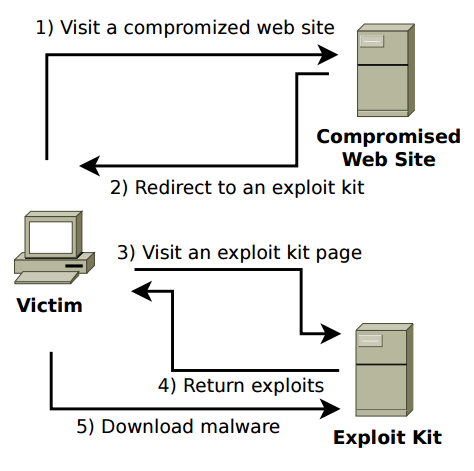
\includegraphics[scale=0.4]{fig/jan-ek-inf}
	\caption{Exploit kit infection scheme from \cite{jan-kotov-ek}.}
	\label{jan-ek-infection}
\end{figure}

\subsection{Institution}%evt. Business?
As a institution or business there are a few ways to reduce the risk associated with botnets or malware infection, depending on the policy regarding usage of computer resources and responsibility of these, measures may vary from business to business.
Keeping software updated is helpful as mentioned, but application whitelisting is not a new concept \cite{jan-mansfield-whitelist}. Instead of blacklisting known bad things the way a anti-virus solution would work we instead only allow known good applications to run, we see implementations of this in Apples iPhone where only applications approved by apple are allowed to run or in Windows AppLocker \cite{jan-windows-applocker} for windows 7 and newer. By limiting the approved applications for a user or a group of users one can limit the attack surface they expose.
Whitelisting network protocols is another way to limit the impact a botnet could have in network, by only allowing certain protocols to communicate a potentially infected computer may not be able to communicate with its command and control server. Similar to this is the act of network traffic inspection, rule based IDS or IPS solutions can look for known attributes in the network traffic and either block or alert when a match is found, in cases where the traffic pattern generated by the download of the malicious code of the bot is known, one can stop the infection before it happens. 




\subsection{Service provider}
Some botnets use a client-server architecture where several clients, or bots, are controlled by a centralized server. To communicate with these servers today where IP-addresses can change often the botnets will use DNS to figure out which IP-address to contact. Sinkholing is the act where you are deliberately sending the wrong IP-address in response to certain queries and end up directing the traffic from the original command and control infrastructure of the botnet to a server controlled by someone else.
This was used by Stone-Gross et al. \cite{jan_stone-gross} when they took over control of the Torpig botnet for several days in early 2009. Torpig was a botnet delivered through Mebroot, which replaced the master boot record of the infected system, a hard to detect rootkit. Mebroot in itself had no malicious function, but delivered other malware as a service. Torpigs victims where infected  through vulnerable web servers which had been exploited by the people behind mebroot. The victims browser would launch a malicious javascript that had been injected into the vulnerable web server which would perform a drive by download on to the victims system, which would infect the system with the mebroot rootkit and add it to the mebroot botnet, which could then download and install Torpig as a module and add the system to the Torpig botnet. \\


A somewhat controversial case of sinkholing domains associated with malware traffic is the case from 2014 where Microsoft got permission to sinkhole traffic towards several domains belonging to Vitalwerks Internet Solutions, the company behind no-ip, a dynamic dns provider. This was later overturned when the sinkholing proved to affect both legitimate and illegitimate use of the domains \cite{jan-microsoft-no-ip}. 
The use of sinkholing does however depend on the domain(s) being under the jurisdiction of a country that will cooperate with law enforcement in whichever country that is seeking action towards specific botnets and their associated domains. Since many of the command control servers utilize services known as bulletproof hosting this can prove difficult. As with exploit kits, many bulletproof hosters are in countries that are less inclined to act on cybercrime targeting foreign countries, however in july 2016 it was reported that several asian countries met to discuss the potential for forming a "Europol-style agency to fight cybercrime"\cite{jan-asia-europol}.

In Cooke et al.\cite{jan-usenix-botnet} they describe botnets using IRC-traffic, as a service provider this means that a botnet could be detected by inspecting the traffic from a network and look for known attributes belonging to a botnet, for instance IRC commands. By infiltrating the IRC channels used by the botnet one can learn of clients that are infected and by looking for DNS lookups of domains associated with the IRC networks one can find clients in ones network that is infected. IRC traffic is usually unencrypted, but can take advantage of for example ssl encryption to mask its own traffic and increase the technical challenge of detecting the traffic.

As technology evolves, so does the botnets with them,  Stone-Gross et al. \cite{jan_stone-gross} describe a botnet named Storm, that  utilized p2p to communicate. Detecting and stopping traffic from new botnets can be achieved by using honeypots and generating signatures based on observed traffic, this is the objective of Honeycomb project \cite{jan-Kreibich}. Honeypots are systems set up by a security researcher or organization to lure in malicious activity from hackers or automated bots, these often contain intentionally vulnerable systems that often appear to contain sensitive or otherwise interesting data or information, so they appear extra enticing for a hacker. By analyzing the commands and patterns of the traffic and actions perpetrated by the attacker one can learn of potentially new vulnerabilities the attacker attempts to leverage or other information such as command and control servers or just in general what the attacker will attempt to perform on a compromised system.


\subsection{Social network}

As described in \cite{jan-fis} the facebook immune system is a system that uses something they call the adversarial cycle(See figure~\ref{jan-adv-cycle-fis}), where the life cycle of the immune system is laid out.
Defending against a attack has a result that is detected by the attacker which then mutates his attack to counteract the defense mechanism. The goal of the defender is to lengthen the time it takes for the attacker to counter the defense mechanism, this increases the cost of the attacker and thus reduces how profitable attacking the social network is. In the facebook immune system they emphasize targeting features with high cost, due to them being hard to detect or change. This can mean targeting infrastructure such as the hosts IP address which can force them to relocate or use proxy services or it can for instance mean implementing tasks that cant be easily automated or not automated at all. Captcha \cite{jan-captcha} is one way to increase the costs of automation, while there exists services that solve captchas for money they cut into already not so great profits \cite{jan-boshmaf} and increasing complexity of captchas when detecting suspected malicious automated behavior could further increase cost for the attacker.


\begin{figure}
	\centering
	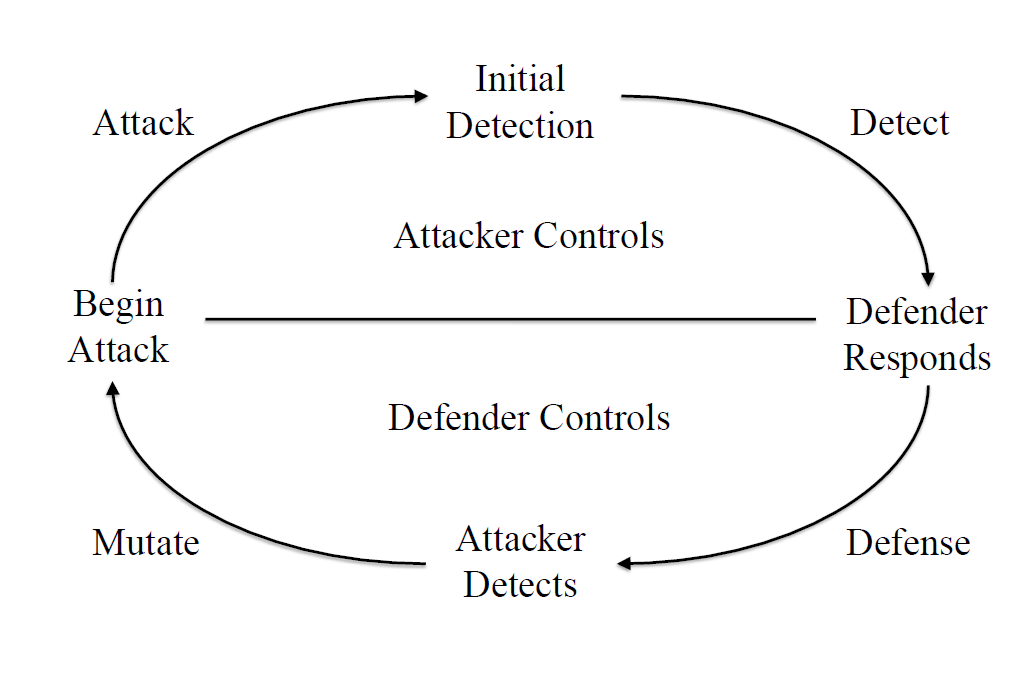
\includegraphics[scale=0.4]{fig/fis-adv-cycle}
	\caption{The adversarial cycle from \cite{jan-fis}.}
	\label{jan-adv-cycle-fis}
\end{figure}
\subsection{Law enforcement and government}
The facilitators of botnets and other malware are in most countries breaking the law with their operation since they are using computer resources without approval of the system owner, it follows that it should be in the interest of law enforcement to stop this activity. 
Due to the international and borderless nature of the internet, enforcing the law on a anonymous person behind a IP address is not a simple task. International co-operation is necessary to effectively take down the infrastructure of a botnet or prosecute the criminals behind it. Many botnets leverage the use of so called "bulletproof hosts" that reside in countries with a legal system that either has no laws at all regarding cybercrime or the laws are simply not enforced in cases where the victim is in another country. Many of these bulletproof hosts will often turn a blind eye towards the legality of the traffic their services are being used for.\\
The Convention on Cybercrime in 2001 attempted to target some of the issues with co-operation between countries and promoting a common criminal policy in relation to cybercrime (\cite{jan-coc}). The European Cybercrime Centre (\cite{jan-ec3}) is a part of Europol that focuses on cybercrime, by promoting cooperation between countries and between law enforcement agencies, private sector and academia.
An example of the results of cooperation between countries in taking down a botnet is seen when the FBI with the cooperation of law enforcement in other countries shut down and arrested the people and infrastructure behind the GameOver Zeus botnet in 2014 \cite{jan-fbi-GOZ, jan-fbi-GOZ2}. GameOver Zeus is p2p botnet targeting windows computers that is based on the code from the Zeus malware, it is thought to have infected up towards 1 million computers across the globe\cite{jan-krebs-goz}. The GameOver Zeus botnet is mostly spread through the Cutwail botnet. The takedown of the GameOver Zeus botnet was a cooperation between government agencies and private software security firms such as Dell, McAfee, Trend micro and many more.
%botnets all the way down.


\newpage
\section{Conclusion}
Depending on which perspective you look at problem from, your available options are different and by themselves they may not be available or be severely limited due to the specific circumstances surrounding your situation. Cooperation between the different groups may overcome this, it should be in the users interest that his place of work is not bothering or hindering his effectiveness in his daily tasks, just as it is in the internet service providers interest to limit the amount of illegitimate traffic going through its networks. Limiting the feasibility of running a botnet can not simply be done by one user, but is a team effort that requires every part of the chain, from the user on his computer to the business in charge of the network to the social network targeted by the botnet.
Increasing the cost while reducing the benefit of running a botnet will eventually make it economically unattractive to run a botnet for criminal organizations

% !TEX encoding = UTF-8 Unicode
% !TEX root = thesis.tex
% !TEX spellcheck = en-US
%%=========================================
\chapter[Social Media Attacks]{Social Media attacks on mobile devices vs. attacks on computers}
\small{By Audun Kjeldaas}
\addcontentsline{toc}{section}{Management Summary}
\section*{Management summary}
\subsection*{Topic}
In this paper I am looking at the differences between the security topography for social media users, on a mobile device, versus that one face when using a personal computer.
\subsection*{Intro}
We have seen an enormous increase in online social media in popularity during the past decade. It has taken over a lot of the networking people tended to do in real life earlier and it makes keeping in touch with a larger network of people a less laboursome task. We tend to trust a friend more than we would any random person on the street and this trust mechanism has been transferred to the cyber space.
\subsection*{The threat picture}
I have found quite a few differences and in other areas the situation is quite similar. The conclusion I reached was that it is, at least at present, much safer to use social media on a regular personal computer than on a mobile device, but that it also depends to a great degree how the user behaves security vice. The share of time people spends on social media networks on their mobile device, versus on their computer, is according to comScore already 79\% vs 21\% \cite{CrossPlatform2016} and still the mobile platform is rapidly gaining terrain. The mobile platforms are getting better protection, but still they are behind on sophistication level when it comes to security. From what I have seen it looks as if you are an easier target for social media attacks when you are using a mobile device, than you are doing the same social media networking on your computer.
\subsection*{How to have a measure of security while still utilizing the potential}
So how do we make sure we are able to maximize the profit from both the mobility and BYOD-trends in the workplace, the increased social network our employees get access to when using social media and last but not least the large, but not so easily calculated, branding value for our business by having a strong presence in social media?
We have to make sure we profit from the positive side of the risk, or opportunity if you want, while at the same time making sure that we have a reasonably secure mobile infrastructure in place. It will never be a good option to withdraw from the use of social media on mobile devices, we would simply lose too much terrain to the competition.
The easiest and most commonplace solution to this problem in the industry today. is to implement an MDMS, a Mobile Device Management System. This will ensure that we can encrypt the work related content on the devices and keep it separated from the personal content the users have. This gives us the opportunity to remotely erase data when devices are lost or stolen
\addcontentsline{toc}{section}{Abstract}
\section*{Abstract}
We have seen an enormous increase in online social media in popularity during the past decade. It has taken over a lot of the networking people tended to do in real life earlier and it makes keeping in touch with a larger network of people a less laboursome task. We tend to trust a friend more than we would any random person on the street and this trust mechanism has been transferred to the cyber space. Cybercriminals, who seem to be mostly concerned with gaining wealth, political high ground, or are ideologically motivated, have shown a keen interest in utilizing these new networking platforms. They come from several different directions, such as attacking via vulnerabilities in hardware, OS, protocols, and apps, but they are also successfully exploiting the trust that exists between members of a social network.
In this paper I am looking at the differences between the security topography for social media users, on a mobile device, versus that one faced when using a personal computer. I have found quite a few differences and in other areas the situation is quite similar. The conclusion I reached was that it is, at least at present, much safer to use social media on a regular personal computer than on a mobile device, but that it also depends to a great degree how the user behaves security vice. The share of time people spend on social media networks on their mobile device versus on their computer is already 79\% vs 21\% \cite{CrossPlatform2016} and still the mobile platform is rapidly gaining terrain. The mobile platforms are getting better protection, but still they are behind on sophistication level when it comes to security. From what I have seen it looks as if you are an easier target for social media attacks when you are using a mobile device than you are doing the same social media networking on your computer.

\section{Hypothesis and methodology}
My hypothesis is that it is easier to attack social media users via their mobile platform gadgets, than via their use of the same media on computers. I have weighed different factors and gathered information around the subject by reading published material saying something about usage pattern, platform weaknesses, distribution of vulnerabilities, and how the users time is divided between the two platform categories. I have looked at how software and hardware protection is being utilized the two cases and I will in the end try to conclude based upon the information presented.
 The subject of social has been moving so quickly, behavioural statistics changing drastically from one year to the next. This constant change makes it difficult to obtain standard peer reviewed research with the latest numbers. For this reason, I have partially leaned on numbers obtained from white papers published by some of the big commercial players in the information security market. These papers are recognized by the industry as reliable sources for such information.
\section{Introduction}
Social media attacks are increasingly common. People’s usage pattern of social media has also changed dramatically during the past few years. An increasing amount of people’s social media interaction is being conducted on mobile hardware platforms. Instead of using Facebook, LinkedIn and other media on the Personal Computer they may or may not still have in their home, they are now using the same media on their mobile devices, such as pads and smartphones. There are also new social media appearing, especially made for these mobile platforms, such as Instagram, which is made to share photos taken with your smartphone on the go.
People now spend more time interacting on social media using their smartphone, than they do using their computer. According to comScore 79\% vs 21\% \cite{CrossPlatform2016}. Since this is a relatively new trend, that has exploded in the past couple of years, it is interesting to see if the migration from one platform to another has led to a more unsecure situation for the users. I limit the type of attack here to direct attacks on end users, with the intension to extract either labour, money or personal data. Nevertheless, I think that the result says something about the security difference we currently have between these two types of platforms.
\section{Attacks on social media users in general}
Some of the most popular social media providers today are Facebook, LinkedIn, Twitter, Google+, YouTube, Pinterest, Instagram, Vine, Snapchat and Reddit. There are myriads more and new services pop up all the time.
While using portable devices to access social media, the user is both a possible target for the same types of attacks that we find being used against computer users and at the same time the limited resources of the mobile devices limits the possibility of using the same advanced mechanisms and software to stay safe \cite{Zonouz2013215}.
Most attacks on the users of these media are economically motivated. There can be different paths to earning money on a social media attack. The reason for an attack can also be politically motivated or even nation state security concerns. There might also be an argument for an attacker to attack via a smartphone instead of a computer because of the potential gain difference. If you successfully own a smartphone you can listen in on the microphone and view the camera outpu as on an owned computer, but a smartphone has a GPS-receiver usually not present in a computer. This GPS-receiver will give the attacker the option to track all the victims movment at all times. In the following subsections I’ll go through a few of the other security conserns and compare possibilities on the different platforms.
As the mobile devices gets ever more advanced and the number of apps, protocols and uses seem to rise towards the sky, it is no big surprise that the number of vulnerabilities follows suit as seen in Figure \ref{fig:mobile_vulnerabilities}.
\begin{figure}
\centering
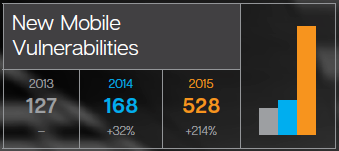
\includegraphics[width=0.5 \textwidth]{fig/mobile_vulnerabilities}
\caption{New mobile device vulnerabilities per year \cite{ISTR2016}.\label{fig:mobile_vulnerabilities}}
\end{figure}
\section{Specific attack vectors for computers}
Microsoft Windows has been the most widely used operating system and thereby represent the largest attackable population. It has also been regarded much easier to attack than the other common computer operating systems, because of the way it is built. 
Apples operating system was long regarded as the safest choice of operating system for a computer, but in the past couple of years there has been discovered many new vulnerabilities and also attack vectors that does not need vulnerabilities to be executed. The fact that this operating system is much less popular than MS Windows also makes it less attractive for an attacker, unless it is directed against a community where Apple products are the most common chiose.
\section{Specific attack vectors for smartphones}
\subsubsection{Android}
New types of attacks are coming all the time. Cross platform attack on Android is being performed via Google Play in a web browser on an ordinary computer. When the victim logs on to the Google Play account on a computer, to install apps on a mobile device running Android, malware on the computer can steal the browser cookies for that session and use it to impersonate the user. It is then possible for the attacker to remotely install apps on the victim’s Android unit. We can also see that the malware is becoming smarter and the sophistication level is rapidly reaching the level of malware for computers. Example are that they are now both obfuscating the code so as not to be detected by malware protection software that uses signatures, and malware that can check if it is running on a real device or a security company’s emulator, thereby avoiding detection. Another weakness with the Android platform is that even if Google pushes out security patches to the makers of all the different devices as fast as they can, many makers take a long time to push these out to their end users \cite{ISTR2016}.
\subsection{iOS}
Apples screening of apps, before letting them into their App store, is very strict, so one can generally be more trusting towards apps found there. Attackers of Apple’s portable devices, running the iOS operating system, for the most had to rely on finding vulnerabilities or attack a jailbroken device to succeed (unlike Android). This is no longer the case. Several new ways of attacking these devices has recently come to light. Symantec mentions two examples of such attack techniques namely XcodeGhost and YiSpectre which can compromise an iOS device without using vulnerabilities or jailbreaking.
\begin{figure}
\centering
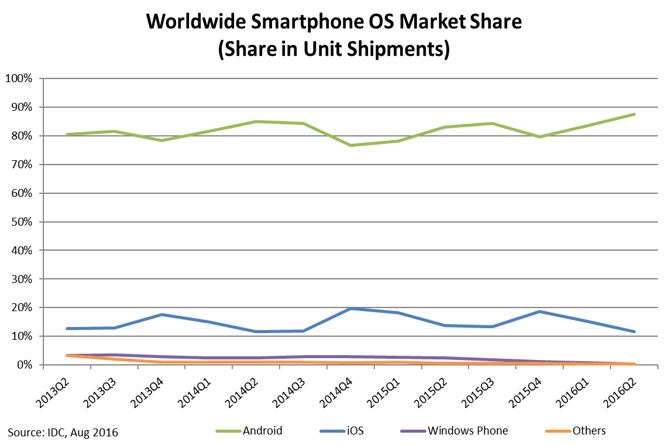
\includegraphics[width=0.8 \textwidth]{fig/smartphone_market_share}
\caption{According to IDC (IDC, Aug 2016) the market share for the Android smartphone OS in August 2016 was 87.6\% And for iOS 11.7\%.\label{fig:smartphone_market_share}}
\end{figure}
The OS distribution in the market means that attackers probably concentrate on Android to get the highest return for their effort. In fact, Kaspersky Lab and INTERPOL has made a report that states that an estimated 98.05\% of all malware is coded to target Android. They also found (in 2014) that the number of detected malware programs for Android had almost tripled since the previous year \cite{Kaspersky2014}. 
\section{Social media attacks directly on the given platform}
There are many ways of attacking social media users/accounts via the platform they are using the media on. There are however a lot of ways to attack via the social media itself, without depending on vulnerabilities in the hardware or software. The attacks simply rely on the many vulnerabilities found in the users, so to speak. These kind of attacks can be based on an account made to impersonate an executive in the enterprise one wants to attack and then build a network of trust by befrending other employees with this account.
\subsection{User behavioural aspects}
Since the name of the game when attacking via social media is trust, it is very important for an attacker to analyse both the company and the specific employees to attack via. The attacker taht wants to succeed in an attack towards an enterprise vill spend a lotof time on social media, logging the victims habits, likes and dislikes, their contacts and if possible what kind of links they like to click on. It is very easy to build a database on a victim just by looking at a n openly available account like Twitter. If you gain access to their Facebook network, for example, you can see what they "Like" and share and easily engineer a spear phishing attack, posing as someone they trust. The behavioural psychology is working against us whan it comes to attacks via social media, our psyhe tells us "this is afriend, someone you know" but unlike when meeting friends for a beer at the local pub, you don't REALLY know who you are communicating with on these platforms.
\subsection{Hardware and software}
The way we use these mobile platforms will largely effect how safe we are from attacks. A lot depends on whether the user installs some kind of antivirus/antimalware program on their device and also how the user thinks about security, compare to when using computer.
Many users leave the Wi-Fi on all the time. It is convenient to have your device connect automatically to all the networks you use, but this convenience comes at a high cost security wise. It is increasingly easy to attack these users by setting up a portable “Wi-Fi-box” that answers the unknowing smartphone owner’s device’s call for a named network, saying “Yes, here I am, please connect to me”. Such devices can be bought readymade on the Internet; an example is the Wi-Fi Pineapple (https://www.wifipineapple.com/).
The other radios in the devices, like Bluetooth and NFC, are also possible entry points for an attacker. We have seen attacks lately using NFC-code stickers containing malicious code or pointing the device user to a malicious website. These stickers can be bought for less than a dollar, programmed via a smartphone and printed with for example “Scan to get 100 free Instagram followers” or something to get people to scan it. An example of a possible attack could be to make the sticker point the user to a mock-up web page that looks like Instagram and since they already think they are there to get more followers they wouldn’t react on having to enter their username and password. 
\subsection{Social media network trust}
People build their social networks online, for most, as they do in real life. They either do know or at least feel they know the people in their social media network to a certain extent. This again leads to trust. People tend to trust the people in their social media network, just the way they trust their friends and co-workers’ in real life.
This trust makes the users easy prey to attackers making it look like links and other things has been sent to them by someone in their network. This can be both sent directly as a personal message, shared to all friends or simply liked. The most popular form of social media scam is manual sharing. Manual sharing consists of something that looks great in some way so that users themselves will want to share it with their friends, like for example a cool video or the chance of winning a new car if you share the post.
\begin{figure}
\centering
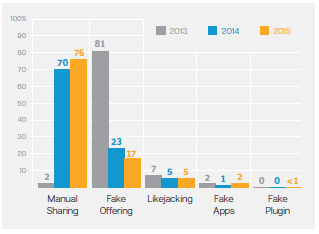
\includegraphics[width=0.5 \textwidth]{fig/social_media_scams}
\caption{Social media network scams by popularity \cite{ISTR2016}.\label{fig:social_media_scams}}
\end{figure}
The mechanisms of these scams works the same regardless of platform, since they are relying on the intended functionality of the app or web page. There should not be any difference in the way people
\section{Conclusion}
Based upon the material I have reviewed I would have to conclude that it is much easier to attack social media users via their portable devices, than it would be to attack their computer. The main considerations behind my conclusion are the following: The majority of time spent on social media is spent accessing these on a mobile device and not a computer. Very few people install any form of malware protection on their mobile devices, while a good majority installs malware protection on their computers. The malware protection solutions that exists for mobile devices, are inferior to the systems available to do the same task on a computer. The number of vulnerabilities found for mobile devices per year is rising quickly. People tend to walk around town with Wi-Fi, Bluetooth, and NFC turned on for anyone to exploit.
So the advice to the general public should be to at least install some sort of malware protection on all their devices, don’t leave Wi-Fi, Bluetooth or NFC on when it is not in use.
% !TEX encoding = UTF-8 Unicode
%!TEX root = thesis.tex
% !TEX spellcheck = en-US
%%=========================================
\newpage
\chapter{Approaches for Detecting Robots \\ in Social Media}

\section*{Management Summary}
Social media platforms, like Twitter or Facebook, are a vital part of the Internet of today. Social bots are programs, that automatically take actions on those platforms. Among other things, they are used for a variety of attacks that, for example, aim to simulate a broad natural support for an entity or to cover unpleasant facts or opinions. Because of that, the detection of malicious social bots is an important task.

This chapter focuses on approaches that can be used in order to detect social bots. These approaches can be classified in social network based, crowd-sourcing based and feature based. Each of these classes is discussed in detail.

Social network based approaches model the social media platform into a graph that describes the relationships between all users. Based on those relationships they try to decide whether a user is a bot or a legitimate user.
Crowd-sourcing based approaches leverage the social competence of actual humans to decide whether a given user is a bot or not. The decision is based on all visible actions of a user. 
Approaches that are feature based make use of machine learning, where a system is trained with known data. During this learning phase, it analyzes which features of user activity indicate a real user or a bot. Afterwards, it uses this knowledge to decide on real data.

It is found, that all approaches have their weaknesses and problems. In order to overcome these, it is advisable to combine different approaches. In addition, it is important to conduct further research in this topic, since the number of social bots is to be expected to continue growing. Also, the developers of social bots will develop more and more sophisticated methods to make their bots appear human and defenders should be prepared for this. 


\newpage
\section{Introduction}
Social media is an important part of today's Internet.  Of the approximately 3.4 billion internet users, about 2.3 billion, that means almost 70 percent, use social media actively \cite{insight}. Especially in order to obtain information about events and the like, social media is often irreplaceable.  For some people social media platforms even substitute real life personal contact to a large degree.

With this importance of social media platforms in the lives of so many people, they get more and more interesting for people that want to benefit economically from them. These are for example companies that want to promote their products and services via social channels. However, the problem here is that, due to their size, it is hard to disseminate a certain message on social media platforms. Like in many other areas of today's  information technology, big data is a huge topic in social media.

This is one of the reasons, why social robots, in the form as we know them today, have been developed. As software robots are often simply called bots, we will use the term social bot or simply bot in the following synonymously for social robot. The propagation of such bots has reached a remarkable high level. In 2014, the social media platform Twitter stated in a report to the United States Securities and Exchange Commission that up to 8.5\% of their active user base may be social bots\cite{twitterbot}.  We will see in the upcoming chapters, that they are used to spread certain messages, to hide others or simply to give the impression of a much bigger support for a person, thing or belief than there actually is. Social bots are also used to directly attack other, actual users, for example to steal their personal data.

First of all, we will take a look at the definition and history of social bots, in order to clearly define what we are talking about and where it originates from. We will then introduce the online social media platforms that are important for this chapter, namely Twitter, Facebook and Renren, and give a short overview about their characteristics relevant here. Afterwards, we will motivate why social bot detection is actually important. In the main part of this chapter, we will introduce several social bot detection approaches and give examples for them. In the last section we will finally summarize our findings and give an outlook about the further developments in this area.

%	\item https://sysomos.com/inside-twitter/most-active-twitter-user-data 32\% of tweets by bots!

\section{Definition and History of Social Bots} 
This section will introduce the term social bot formally and give a short overview about the beginning and the development of this topic.

In order to be able to discuss social media bot detection, we need a clear understanding of what social bots actually are.  For that, we use the definition given by Ferrara et al. in their article The Rise of Social Bots:
\begin{quote}
	"A social bot is a computer algorithm that automatically produces content and interacts with humans on social media, trying to emulate and possibly alter their behavior." \cite{ferrara15}
\end{quote}

A social bot is therefore basically any software that acts as a user, or something similar, on social media platforms. As the broad definition suggests, they can appear in many shapes.

The root of of social bots, can be found in the Turing test, developed by Alan Turing in 1950 \cite{turing}. It involves three parties, two of them are human and one is a computer program. While one human is having a conversation with the software, it is the task of the other human to identify the program by looking only at the conversation. If he is not able to do so, the software is passing the Turing test. This led to the development of a lot of so called chatbots, which just aimed to appear as human as possible in a conversation.  

A rather famous and often cited example for such a chatbot is ELIZA, introduced by Joseph Weizenbaum in \cite{eliza}. It mimicked a psychotherapist and showed that, at least some kind  of, communication between a human and a computer is possible.

Since then, a lot of things have changed. Today, bots are a lot more than bare entertainment or proof of concept. With the triumph of the Internet and especially social networks like Facebook and Twitter, the possible use cases for social bots have increased dramatically. While they were initially mostly used to simply post content, today they are able to credibly interact with each other and even humans \cite{boshmaf13, hwang12}. As we will see in the next section, nowadays' bots are used to spread messages, for marketing and a lot more.

\section{Important Social Media Platforms}

In this section we want to give a short overview about the social media platforms, or online social networks (OSNs), that are relevant for this chapter. This is necessary in order to better understand the problems and attacks that will be presented later on. However, we will describe those networks only as detailed as necessary in this context, since a thorough explanation would go beyond the scope of this chapter.

The first and probably most important OSN that needs to be mentioned here is Twitter\footnote{https://twitter.com/}. Twitter is a microblogging network which allows its users to broadcast short messages, so called tweets. Tweets are delivered to anyone that follows the tweeting account. Following is hereby a one-way process, that does not need any confirmation by the followed account. To see the tweets of a certain account, following is not necessary though. Thus, tweets can be regarded as public. Furthermore, tweets can be retweeted. Retweets can be seen as a forwarding of a tweet in order to disseminate it: all followers of the retweeting account get the retweeted message.  Tweets can be tagged with hashtags, that associate them with a certain topic or an ongoing discussion.

Another OSN that is important for this chapter is Facebook\footnote{https://www.facebook.com/}. As on Twitter, it is possible to publish messages on Facebook. However, the visibility of those messages, or posts, can be adjusted. Usually, posts are only visible to users that are friends with the posting account. A friendship is here, in contrast to follow-relationship on twitter, bilateral: a user can send a friendship request to another account which has to accept it in order for the relationship to be built. Another important difference to Twitter is, that Facebook accounts respectively profiles usually contain a lot more personal information than Twitter accounts do. Like it was the case with posts, the visibility of Facebook profile pages can be adjusted and usually they are only visible to accounts that are friends.

The last platform we want to mention shortly is Renren\footnote{http://renren.com}, which is a chinese OSN directed mainly at college students. Like Facebook it uses the concept of friendships and highly personalized profiles. It also allows to post messages that can be seen by friends.

\section{Why is Bot Detection in Social Media Important?}
Another point that is important to be looked at before we go into detail about the actual detection methods is, why social media bot detection is important at all. In this section we will argue, why this is an important topic, especially today. 

As already said above, social media platforms are nowadays an important component in the life of many people. For some, they even substitute real personal contact sometimes. Thus, it is important to ensure, that humans are still able to estimate what is happening in their social media surrounding and what can be seen as trustworthy -- and what cannot. While the challenge of verifying facts or news from the Internet is not new, social bots add a new factor to this challenge. They can make a non-trustworthy source look trustworthy by simulating that it is highly popular.

An example for this, is the so called astroturfing. In an astroturfing campaign, an attacker tries to give the impression of a broad grassroot support for a certain person, belief or political position. A known political astroturfing case are for example the 2010 Massachusetts senate elections in the US. During these, a small number of Twitter social bot accounts produced a large amount of tweets that contained a link to a website that smeared one of the candidates. The tweets also mentioned users that had shown the same political position beforehand and thus were likely to retweet. In a few hours the smearing website link spread rapidly what was even noticed by the Google search engine. That way, the website got promoted to the top search results for the name of the smeared candidate \cite{mustafaraj10}. 

A similar approach can also be used to distract from potentially inconvenient or just unwanted facts or opinions is called smoke screening. By just flooding the platform with information, it aims to draw attention away from the unwanted topic to a topic that suits the attacker more. The flooding information can hereby even be related to the topic that is to be screened. It just focuses on a component that is more pleasant to the attacker and withholds the inconvenient part. An example for this is given by Abokhodair et al. \cite{abokhodair} in the context of the syrian civial war. They analyzed a social botnet on Twitter from April until December 2012. It made heavy use of this technique in order to cover up news about the civil war in Syria.

Another, more direct, example for an attack scenario is described by Boshmaf et al. \cite{boshmaf13} They operated a network of social bots on the social media platform Facebook and successfully tried to build as many relationships as possible with real users. After this was done, they were able to extract data from the profiles of those real users that were not publicly available, like for example mail addresses or phone numbers. While they show that operating such a botnet for the sole purpose of data extraction might not be efficient for an attacker, they argue that this data can be used for more advanced attacks afterwards.

Besides all these specific attacks, which are carried out by bots built for this purpose, there are also simple negative effects from social bots that have not necessarily been built for an attacking purpose.
The information in social media is often used by various entities. An example for this is the area of emergency response. By analyzing the information streams of social media platforms it is possible to estimate emergency situations and to take proper actions for decision makers. Cassa et al. \cite{cassa} for example show, that information about the Boston Marathon attacks in 2013 was more than five minutes earlier available on Twitter than the public health alerts, even though there were already many first responders present on this event.  Another area where information from social media platforms is leveraged is the stock market. By monitoring the general mood on Twitter, for example, it is possible to predict the market trend to a certain degree \cite{bollen}. A case can be made that this is also already done by traders. When in 2013 for example the Twitter account of the Associate Press was hacked and it posted rumors about a terrorist attack, the stock market crashed significantly \cite{ferrara15}. It is therefore not hard to see that bot-caused information distortion on social media platforms -- that does not even necessarily needs to be intended malicious -- can have severe impact. Some social bots are built just to retweet and if they retweet false information or rumors they help to make this information popular. This happened for example also after the former mentioned Boston Marathon attacks, where false accusations were spread by such social bots \cite{gupta}. 

Furthermore, social bots are often used by public persons in order to appear more popular and thus to gain influence or by companies in order to promote their products on social media platforms \cite{stringhini}. Here, social bot detection is necessary for ordinary users as well to be able to distinguish between real and bought support.

%---> section "engineered social tampering" and following in the rise of social bots!! 

%\textbf{Im Prinzip angriffsübersicht?}

%+ Key Challenges in Defending Against Malicious Socialbots \cite{boshmaf12}


\section{Social Bot Detection Approaches}
In this chapter we want to introduce several techniques for detecting social bots. Based on Ferrara et al. \cite{ferrara15} we distinguish three detection approach classes. 

The first category of detection approaches is based on social network information. They are also called graph-based, since they map users and their relations into a graph and then try to identify bots in the hereby obtained social network by means of graph theory. 

Afterwards we will discuss crowd-sourcing based social bot detection approaches. They use actual humans to detect bots, assuming that the human ability to notice details in communication will make this an easy task.

The last category we want to elaborate on are detection approaches based on behavioral features. Mechanisms that make use of this approach try to observe behavioral patterns that are typical for humans and social bots. By doing so they aim to distinguish bots from human users. 

In the following sub sections, we will go into detail about each of these three approaches and illustrate them using real detection systems. It has to be noted though, that the borders between the individual approaches is not always very clear, so that some examples could also be mentioned in a different category. Many schemes for example, use some kind of graph theory. However, we try to categorize them by their core traits.

\subsection{Based on Social Network Information}
A term that is often used in combination with detection of bots by using social networks is sybil or the sybil attack. It was presented as a thread to distributed systems by John R. Douceur \cite{sybil}. In the specific context of social media platforms, when conducting a sybil attack, an attacker creates a large amount of fake identities in a system to the point where these identities make up a considerable fraction of the system's whole user base. When this is achieved, the attacker can influence the whole system and control its contents to a certain degree. A sybil, sybil node or sybil account is therefore simply one of the fake entities, or depending on the attack's architecture, just a social bot. It is not hard to see that social bot detection can, more specifically, be viewed as a defense against the sybil attack.   

The general proceeding of bot detection approaches based on social network is rather simple. They map the user base of the OSN they aim to defend into a social graph, where a node is corresponding to a user and an edge between two nodes exists if there is a specific kind of relationships between the two respective users on the platform. The nodes can hereby be distinguished in sybil nodes, respectively bots, and non-sybil nodes, respectively legitimate users. The goal of the detection approach is now, to identify whether a given node is a sybil or not \cite{comparison}.

There are a number of proposed social network based sybil detection schemes like for example SybilGuard \cite{sybilguard}, SybilInfer \cite{sybilinfer} or SumUp \cite{sumup}. While they all have different assumptions and use varying algorithms to achieve their goal, Viswanath et al. \cite{comparison} show that, at a high level, all of them work by them same principles.

Basically they can be viewed as graph partitioning algorithms, which partition a given graph into multiple disjoint subgraphs. As already mentioned above, ideally two subgraphs are assembled, one that contains only sybil nodes and one that contains only non-sybil nodes. Since a clear distinction is often hard to make, the approaches basically assign a rank to each node and decide afterwards, depending on several parameters, which ranks are classified as sybil and which as non-sybil. It is thus obvious, that the ranking algorithm is crucial for the whole scheme. Although, of course, the ranking algorithms for the different detection schemes are different, they generally have in common, that they base their rating on how tightly connected the respective node is to a known trusted node. Thus, they work by detecting local communities of nodes, in other words closely connected groups of nodes \cite{comparison}.

It is not hard to see, that these algorithms are therefore easy to deceive. If an attacker is able to establish so called attack edges, connections between his sybil nodes and non-sybil nodes which are connected to a trusted community, it gets significantly harder to identify the bots. A common assumption is that these attack edges are hard to create \cite{sybilguard}, which means, that legitimate users tend to not establish social network connections to social bots. However, Boshmaf et al. show \cite{boshmaf11} that this assumption is to be questioned. 
They tried to infiltrate Facebook with a large number of sybil accounts and to establish connections to real users. The average acceptance rate of their friendship requests came to about 20\% and could be increased to 80\% depending on how many indirect friendships between the sybil and the user already existed \cite{boshmaf11}.

A well known example for a bot detection approach that is based on social network information is the Facebook Immune System (IMS) \cite{fis}. This system aims to defend the social media platform Facebook and its users not only against sybil attacks but also to prevent spam, malware distribution, phishing and so on.  To achieve this goal, it takes a lot more actions than the above described general approach for social network based detection schemes. The IMS runs checks on every action performed on Facebook in realtime in order to give attackers as less time as possible to accomplish their goals and to react. It classifies these actions according to predefined policies and makes it thereby possible to judge them and the corresponding users.

An example for this could be a newly created Facebook account, that sends a lot of friendship requests. A legitimate user starts sending friendship requests usually mainly to people he knows and vice versa, that is, people that are likely to accept his friendship request. If a lot of these requests are now declined, this could be a indication for the system that the sending user might not be legitimate.  The IMS also makes heavy use of machine learning, to which we will come back in later on, and generates training data automatically in order to adapt to the fast changing attacks and user behavior.

\subsection{Based on Crowd-Sourcing}
A rather straight forward approach for social bot detection is based on crowd-sourcing. In contrast to the above described social network information based approaches, a connection between bots and legitimate users is not a problem for schemes based on this approach -- at least not a direct one. The basic idea of crowd-sourcing based social bot detection is, to engage actual human workers to study user profiles and subsequently to decide whether it belongs to an actual user or a sybil.

Wang et al. \cite{wangcrowd} present a study on the effectiveness of this approach and introduce a sample for a crowd-sourcing based social bot detection system.  For their tests they use data from Renren, China's most popular social media platform, Facebook US and Facebook India. They subdivide their human investigators, or simply testers, in expert workers, and crowd-sourced workers.  Each of the testers is presented a number of social media profiles and has to decide, whether it is a real one, or a sybil. While the experts achieve a detection rate at about 90\%, the crowd-sourced workers perform not as well individually. If their single votes are aggregated and used for a majority decision though, the results can be significantly increased. If this is done for the expert workers, their results can be increased even more, too. A very desirable result of their studies is also that the false positive rate, that is the amount of profiles that are falsely classified as sybils, is in all groups very close to zero. This ensures, that the probability that legitimate users are accused to be social bots, what will probably offend them, is very low.

Wang et al. conclude, that it is very hard for sybil creators, to assemble social bots, respectively profiles, that are able to pass a "social turing test" and that crowd-sourcing based approaches can perform very well. They proceed with introducing a general practical system that is illustrated in figure \ref{crowdsys} \footnote{Turkers are in this case the former mentioned crowd-sourced workers.}.

\begin{figure}
	\centering
	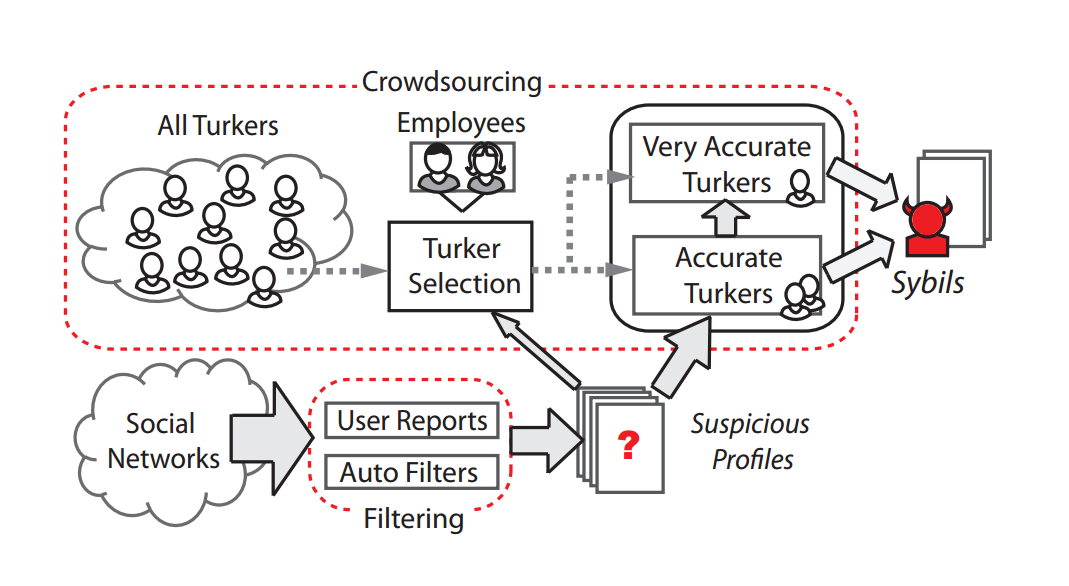
\includegraphics[scale=0.4]{fig/crowdsys}
	\caption{A crowd-sourced sybil detection system introduced by Wang et al. \cite{wangcrowd}.}
	\label{crowdsys}
\end{figure}

The system works like this: The social network that is to be defended generates suspicious profiles. This can either happen through explicit reports from users or through automatically applied filters that detect abnormal behavior. The so obtained profiles are then checked by crowd-sourced workers, which are subdivided in accurate and very accurate. To establish this differentiation, some of the suspicious profiles are mixed with some profiles that are known to be sybils. They are presented to all workers and their results allow a classification and to filter out unreliable workers. In the actual checking process, the profiles are first presented to the accurate workers which make a majority vote. If their decision is not clear, the profiles are presented to the very accurate workers which once again make a majority vote. 
The authors claim, that a system like this is very reliable and cost effective. 

Although such a social bot detection approach based on crowd-sourcing seems very promising at first sight, several problems become obvious on closer examination. First of all, this approach works optimal if every newly created profile can be reviewed in the above described way. However, young social media platforms will probably not be able or willing to pay for this bot detection scheme. A factor that may influence this could also be, that those platforms probably do not have huge issues with the social bot problem in their early stages. Once the platform has grown and the issue arises though, their is usually already a huge user base that has to be reviewed retrospectively. This is not optimal and may take a considerable amount of time.

Another point that must be taken into consideration is that this approach might not be suitable for all types of social media platforms. While it might be well suited for platforms like Facebook or Renren, where profile pages can be customized a lot and contain usually plenty of information, other networks, like for example Twitter could be less appropriate for this approach. Generally it can be said that this detection approach is highly based on the information given in the users' profiles. If the information contained in the profiles is low, human investigators will probably not be able to distinguish as precisely as in the tests of Wang et al.

The last and probably most difficult issue that has to be mentioned is connected to this. Human investigators that are charged with distinguishing between bots and legitimate users need to have access to the profiles of the users. While those profiles are sometimes publicly available anyways, detailed profiles, which are more interesting for this approach, are, as discussed above, usually only visible for certain users. It is not hard to see the privacy issue that arises here, especially when keeping in mind, that the investigators are -- at least to a great extent -- only crowd-sourced workers, that cannot be supervised as easily as ordinary employees \cite{ferrara15}.


\subsection{Based on Features}
The last detection approach for social bots is based on features. Features hereby mean observable characteristics of posted information, profiles and possibly anything else that can be associated to the account in question. Schemes that make use of this approach often use machine learning algorithms. These are algorithms that are able to make decisions based on learned patterns. They basically consist of two phases. In the first phase, the so called training phase, the algorithm processes training data which is labeled with the decision that should be made on this piece of data. By processing a lot of training data, the algorithm learns the features that are indicators for a certain decision. In the second phase, real data is processed and the algorithm is able to make decisions based on the learned data. Thus, schemes that make use of this detection approach can be compared to anomaly based intrusion detection systems. In the social bot detection topic, the decision being made is usually whether a specific account is controlled by a bot or a human. Since it is not easy to make a clear decision in many cases, there are often multiple decision options that each express a degree of certainty.

A well known example for this kind of social bot detection is the Bot or Not? system, presented by Davis et al. \cite{botornot}. It is a publicly available\footnote{http://truthy.indiana.edu/botornot} system that allows a feature based social bot detection for accounts on the social media platform Twitter. Bot or Not? was trained with about 31000 account samples of both, human and social bot accounts. For classification, it makes use of more than 1000 features that can be assigned to six feature-classes. In the following we want to mention these classes shortly:
\begin{itemize}
	\item \textbf{Network} features reflect on the spreading of information, for example citations of different users or the like.
	\item \textbf{User} features take the information given in the actual account into consideration. Meta-data, that is basically data about data, is especially relevant in this feature. 
	\item \textbf{Friends} features are about the social relationships of the account in question.
	\item \textbf{Temporal} features analyze issues like the rate in which content is produced and the like.
	\item \textbf{Content} features are about wording characteristics in the texts produced by the relevant account.
	\item \textbf{Sentiment} features reflect on emotional aspects and are obtained by using specific algorithms \cite{botornot}.
\end{itemize}  
If a Twitter account name is entered in the Bot or Not? system, it checks all of those features and afterwards decides, based on the former mentioned training data, whether this account is a human or bot account.

Another social bot detection approach that can be classified as, feature based relies on detecting the coordinated behavior between social bots. Schemes that make use of this approach focus generally on the above described network, content and temporal features and often incorporate some graph theory as well. They usually aim at detecting attacks which try to distract from unpleasant facts or to distribute fake facts, like in the above described astroturf attack.  An example for such a scheme is SynchroTrap, presented by Cao et al.  \cite{synchrotrap}. Again, comparable to anomaly based intrusion detection systems, SynchroTrap makes use of clustering algorithms. These algorithms try to group values, that are similar in some aspects into distinct sets. 

The system monitors all user activity on a social media platform over an extended time period and monitors aggregated user actions. Then, the pairwise similarity between actions is determined and a hierarchical clustering algorithm is used to group users that show similar behavior at approximately the same time. If a cluster is growing too big, it can be assumed as malicious, since legitimate users tend to behave diverse \cite{synchrotrap}.

An issue of this detection method is though, that it is for example not able to detect bot accounts that show a mixture of bot and human behavior. Thus, the detection systems have to be developed further in order to keep up with the fast evolving social bots and their evermore sophisticated behavior \cite{ferrara15}.


\section{Summary and Outlook}
In this chapter, we firstly introduced the term social bot, defined it and looked at the history of robots in social media.  We also gave a really short overview about the OSNs that are most important for this chapter and motivated why social bot detection is important after all. Mainly, we discussed social bot detection approaches. We distinguished hereby social network information based, crowd-sourcing based and feature based approaches. 

Social network based approaches model the analyzed OSN into a graph where users correspond to the vertices and relationships between the users correspond to the edges of the graph. Afterwards, an algorithm tries to make a decision whether a given node is a social bot or an actual user. A problem these systems have to cope with is, that they tend to assume, that bots can't establish relationships to actual, what emerged to be false.

The basic idea of crowd-sourcing based approaches is, to engage actual humans to analyze given user profiles and to decide whether they belong to an actual user or a social bot. We discussed a paper which analyzes this approach thoroughly and introduces a general practical system. One of the issues this approach has to handle is that some social networks users don't have very detailed profiles what makes crowd-sourced bot detection very hard. 

Feature based social bot detection approaches observe characteristics of OSN users and information published by them in order to decide -- or give a tendency -- whether a given account is a bot or not. Often, they make use of machine learning algorithms. 

After analyzing the different detection approaches, it becomes apparent that each has its own problems and a combination of different approaches may yield good results. Observing the social graph and behavioral features of accounts together is for example a promising strategy. Ferrara et al. \cite{ferrara15} bring in the Renren sybil detector \cite{wang2013, yang2014} as a good example for these combined approaches.

However, it has to be noted that not all robots in social media have to be evil necessarily. Some social bots provide useful services that many users do not want to miss. It is just important, that users are able to distinguish between other humans and bots for example in order to differentiate whether content they see is actually as popular as it seems.

It is safe to assume that the number of social bots will increase even more and that their methods and behaviors will get even more sophisticated. We expect an arms race between bot herders and bot detection mechanisms, like it was -- and still is -- the case with malware and malware detection software.


% !TEX encoding = UTF-8 Unicode
% !TEX root = thesis.tex
% !TEX spellcheck = en-US
%%=========================================
\chapter[Bot Metrics]{Do bots,  make click, text and behavior metrics irrelevant?}
\section{Management Summary}
In todays society, where everyone has a online presence, and many of our financial transactions are based on online content, one has to maneuver smartly through the grapevines which makes up the internet. In the article we find examples that many costumers buy based on recommendations, and reviews alone, and are therefore prone to being manipulated by fake content like bot metrics. In the 2014 Superbowl, people were in general tweeting more during the commercials than they were during the games. If bots also interact in this, we can safely say that these types of interactions can influence what we buy and why. 
It is not only through financial transactions bots have entered the fray, its also in society in general. In the 2016 U.S election, research shows that about 400 000 bots influenced the election on Twitter, giving rise to the claim that we may be influenced by non human entities, and that this might have had some deciding factor. The article includes research about how bots are perceived by humans, and shows that they found the Twitterbot in this case very trustworthy, which reinforces the thought that bots and their actions might implicate us in a larger manner than what was first believed. We discuss how the metrics influence us through direct examples and their implications. The article concludes that bots will always be a part of the metrics, because bot detection is a very complex problem which cannot guarantee a 100\% bot free environment. 

\section{Abstract}
This article will focus on bot metrics used in E-commerce(social media analytics), as well as bot metrics in other commercial contexts. According to research which will be presented in this article, bots are used in numerous ways, from rigging elections, hiding its own purpose by masquerading as users, to spreading misinformation from unverified sources, to promoting sales as well as working as sales representatives in e-commerce. This article then tries to delve into metrics by looking at social media statistics(SMA) in order to highlight why it may be worthwhile to fool the metrics and further uses a real world example in the case of IMDB reviews in order to give an understanding of how metrics in worst case could influence a buyers' decision, as well as how metrics in the U.S 2016 elections might have been a deciding factor for some twitter users, affecting the outcome of the election. The article is concluded by a discussion on whether or not bot metrics in behavior metrics cause metrics themselves to be irrelevant. 

\section{What are bots and how are they used?}\label{intro:howwhenwhy}
In general, bots are types of software which run automated tasks(which are repetitive and allows for the program to be faster at doing some tasks than what normal humans would be able to. There are many types of bots, for example gaming bots which can be programmed to efficiently react faster than what a human would be able to on certain events in the game, thus making the humans better players. Others examples include auction bots, which hunt for bargains. Ebay went to court in 2000( \cite{Computerworld:Ebay}) in order to stop this type of behavior, the federal courts in turn then decided to block Bidders Edge and their bots from accessing Ebays API.
\\

In the US 2010 mid-term election, social bots were reportedly used to influence the support of some candidates while effectively slandering others by tweeting thounsands of tweets which pointed to websites which contained fake news about the other candidate (\cite{ICWSM112850}). This example highlights the potential seriousness of social bots. \label{midtermElection}
\\
It is not only in elections these bots have a great influence, during the aftermath of the Boston bombings it was noted that social media(and bots) had a great effect on getting the message out there(\cite{Cassa:Twitter}), but there was also a negative effect which bots attributed on Twitter by re-tweeting peoples' unverified accusations or even checking out the credibility of the source, causing more hurt than good. \\
\\
Furthermore bots are used to mimic human activity, in for example service applications which appear to be human interaction but is instead a bot which for example tries to "help" you based on keywords. Bots are used in many areas, but are probably most known for their maliciousness in areas such as spam, bandwidth-thiefs, scrapers, worms and viruses as well as as nodes in a larger scale bot-nets is used for example for DDOS. These bots can be part of bigger bot-nets in order to for example generate revenue through for example click fraud. 
\\
\\
The observers article on fake traffic \cite{Observer:FakeTRAF} describes the problem and its extent: 
\begin{quote}
A recent study by comScore found that 54 percent of display ads shown in thousands of campaigns between May 2012 and February 2013 never appeared in front of a human being. Rather, the traffic came from bots. As an advertiser, this would be like buying a billboard you were told was seen by thousands of cars a day only to find out that was because the billboard sat next to the assembly line at a Ford plant. Sure, that’s a lot of cars, but there’s no one in them.
\\
\\
In fact, the system is so broken that, for some publishers, knowingly buying traffic that comes from bots is part of their business model. An anonymous publishing executive, who claimed to be buying up to \$35,000 worth of traffic per day, recently told Digiday that for publishers running an arbitrage model, all that matters is profit; quality of traffic does not factor into the equation.
\newline 
\mbox{} 
\hfill 
\cite{Observer:FakeTRAF}
\end{quote}

This quote from comScore highlights a important point in today's society. How does click metrics influence us, and how are they used? Are they useless, can they be used to measure something even though results most likely have been contaminated? and how does this type of behavior influence the buyers decision? These and some others are the question I will answer during this chapter. 


\section{What is  social media statistics, and how is it utilized?}\label{intro:howUtilized}
With the rise of social media use, social media marketing got a bigger foothold, allowing marketeers to interact with their buyers to a bigger degree, and it allowed the buyers to interact with their brands. Following this trend, many companies have big social media presences. Social media statistics allows the companies to closely monitor and narrow down their demographic and easily make specific content for a specific demographic. Furthermore, it allows for the company to get free publicity through what is called "organic reach" (getting exposure through users' activity in order to generate more clicks from users' contact) as well as for example paid reach(ads sent to a predefined demographic)
Social media statistics allows for all of this to happen, as \cite{Singh2013} mentions:
\begin{quotation}
Social Media statistics about audience likes and dislikes makes it plausible to employ "push marketing"-techniques to target audiences with advertisements that are relevant to their interests. Also, parameters such as click through rates or CTR can further quantify the success (or failure) of an advertising campaign. 
\end{quotation}
This type of push marketing, utilizes the information the users' themselves have provided to the mother service(e.g. Facebook), like for example metadata which gives a certain characteristic which allows them to be targeted by the broad filters which services like e.g. Facebook uses. 
\\
Businesses also utilizes what is called pull marketing, which is a little more subtle, e.g. referrals, social competitions("like and share" and get the \textit{chance} to win X") these methods can generate traction in social media, and be spread by word of mouth. 
\\
\\
But most notably, these types of metrics can be obfuscated by bots, masquerading as real users. These types of metrics can be abused by bots because bots are hard to detect using convetional statistics and other methods, in an article entitled "Fool Me If You Can: Mimicking Attacks and Anti-Attacks in Cyberspace" \cite{6601602} researchers establish that legitimate cyber behavior can be simulated, and further that it cannot be discriminate mimicking attacks from legitimate cyberevents, in the case of big bot nets. Furthermore, the article concludes that conventional staticial approaches such as viewing time interval and browsing length, can be easily mimicked if this data already exists. This all highlights the problem with bots.


\subsubsection*{An example of why metrics may be come obfuscated}\label{obfuscatedmetrics}
What happens to social media analytics in a business environment when bots enter the fray? Depending on the function of the bot, its behavior can vary greatly. If the bot is what is called a crawler, the bot will crawl through real peoples feed and try to mimic their behavior, and then crawl and gather more data from other people in the first peoples feed and so on. This type of activity has atleast three types of repercussions, it firstly generates fake interest for other companies' social media analytics, it hides their original intention(liking "this page") and it likes "this page" and generates fake revenue and publicity.
\\
\\
\label{Symantec:mockingbirds}A good real-life example is \cite{Symantec:Narang}, which had a set of inter chained accounts posing as real accounts in order to spread their own links about some dubious diet pills. The accounts stole meta data from real accounts. Instead of using compromised
accounts to tweet spam links, they were using accounts that impersonated brands and
celebrities. Symantec goes on to describe how they defined three types of accounts involved in this scam:
\begin{itemize}
\item {\textbf{Mockingbird}: Used real data from real celebrities for impersonating these individuals}
\item{\textbf{Parrot}: Fake accounts using stolen tweets and photographs of real women}
\item{\textbf{Egg}: New users with no set avatar}
\end{itemize}
Mockingbirds have the goal of promoting the weight loss tricks. These mockingbird-tweets would get thousands of likes from Parrot-accounts which spiders through the real accounts of the mockingbirds. Parrots then follow any and everyone in the hope that users will follow them back because they are using avatars of attractive women, a tactic that has proven very efficient. The Parrots have real content that they post each day which is fake, an not only the content of the Mockingbird, in order to seem more real. These tweets are usually stolen from real accounts in order to seem real.  The parrots will also engage in discussions and post "reviews" of the diet pills in order to make the diet pills seem more real while the egg accounts just inflate the like counts in order to make the mockingbirds as well as the parrots seem trustworthy. The egg accounts do not post any content, they just follow parrots.
\\
\\ The link provided by the mockingbirds seem real(with pictures of famous people). When a customer orders a free trial, they register the credit card and subsequently lose their money. 
\\
The point of this example is to show how easily for example likes can be misguiding for a company that tries to establish themselves as a brand within social media. 

\section{Do these metrics influence buyers?}\label{metricInfluence}
As we have seen, metrics can be obfuscated by many different factors; "click farms", bots, and other variables which can affect social media analytics. These factors may present in many different ways. In an article entitled "Beyond likes and tweets: Consumer engagement behavior and movie box office in social media", \cite{Oh2016}, they researched how consumer engagement behavior(CEB) was associated with economic performance based on popular movies released in the US. The study found that CEB in Facebook and YouTube correlated with gross-revenue in opening-week movies. The study further concluded that CEB played a pertinent role in relation to future economic performance, so in some cases pure metrics can have great effects on the consumer itself.
%%
%%
\\\\ Another good example of this is metrics in movies. In particular ratings on movies and Tv-series through IMDB(Internet movie data base), which is used to share users' opinions on films and tv-series in the form of ratings(top 250 movies, bottom 100) as well as recommendations and critics, both professional and user generated. In a paper entitled "Judgement devices and the evaluation of singularities: The use of performance ratings and narrative information to guide film viewer choice"(\cite{Bialecki2016}), the researchers noted that the use of metrics such as ratings(moviegoers set a threshold in which served as a "hurdle" in which movies they wanted to see had to pass). Research also indicated that if a movie had a high rating or were in the top 250 rating-list, it was likely moviegoers would see it because of the ratings themselves. Some subjects noted that the movie did not meet their expectations, but that they had to watch it because of the the ratings:
\begin{quotation}\label{MovieReview}
\textbf{\textit{"}}I rented this movie on the strength of the ratings and glowing
reviews at this site [IMDb]. “Brilliant”,they said. “Dark and beautiful”,
they wrote. 8.4 stars. Well, all I can say is, these people
must have been on some serious drugs when [they] saw this
totally inane movie. . .I give this movie 1 black hole.\textbf{\textit{"}}
\newline \mbox{} \hfill \cite{Bialecki2016}
\end{quotation}

\label{Emil:oogie}
As we can conclude from \cite{Bialecki2016}, we can say that people buy largely based on word of mouth as well as from reviews or "click metrics" (in the form of stars on IMDB). While doing research for this article, I found several websites which both offered botting specifically for IMDB(increase in stars), as well as a direct example of a movie in which had been a "bottom 200-list"-er for a long time, and was considered one of the biggest movieflops, gathering great nominations such as "Worst picture", "worst screen ensamble" \cite{emil:wiki:oogieacc} as well as a IMDB rating of 2.0 according to a petition \cite{Emil:change:Oogieloves}. The petition goes on to describe how the rating of the movie suddenly skyrocketed in June of 2013. in \ref{IMDB:rate} we can see the weighting of votes, most of which are at 10, which is the highest. This seems peculiar given the accolades which the movie was given and the initial score as well as the sudden boom. The ramifications of such actions will be discussed in the discussion part of this paper. 

\begin{figure}[h]\label{imdbratingCurve}
\centering
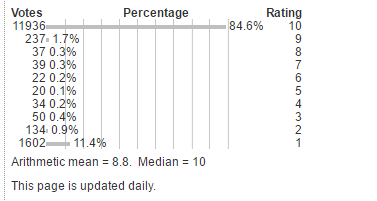
\includegraphics[scale=1]{fig/imdbstats.png}
\caption{IMDB rating of "The Oogieloves in the Big Balloon Adventure" in 2016, showing the skewed ratings.Courtesy of IMDB(\cite{IMDB:Oogieloves})}
\label{IMDB:rate}
\end{figure}

Another example of research done in this field is an article entitled "The Influence of Social Media: Twitter Usage Pattern during the 2014 Super Bowl Game" which analyzed how people used twitter during the superbowl event specifically looking at consumer interaction with advertisement.
The researchers used data mining in order to find correlations in data which may not be otherwise easily delectable. 
In the article(\cite{HyeonjeongShin2015}), the researchers asked two research questions: "How does the overall number of tweets differ between a game day and non-game day?"\cite{HyeonjeongShin2015}) and "What major topics in commercial related tweets were exchanged during the 2014 superbowl game?"\cite{HyeonjeongShin2015}). The data analysed for research question 1 (How does the overall number of tweets differ between a game day and non-game day?) indicated that Super bowl commercials created a buzz. The research also indicated that tweets about a commercial product accounted for 33\% of total commercial tweets generated on superbowl day(february 2) as opposed to 0.64\% and 9.48\% on january 26 and february 9th. Further, more than half of tweets(37 of 49 tweets) registered mentioned Budweiser products or their commercial. 
\\
\\
Even though these examples do not directly prove that consumers act on these type of data, one can draw the conclusion that user interacting might create a buzz and get your brand out there, thus leading to potentially more customers, subconsciously or otherwise. 

In the case of IMDB-ratings, they seem to influence what movies people want to see, and therefore revenue of movies which are featured in a popular way. This is backed up in a article entitled "An empirical investigation of user and system recommendations in e-commerce" about general statistics with e-commerce metrics \cite{Lin2014111} which could report that:
\begin{quote}
\begin{itemize}\label{userreccommendation}
\item {1\% increase in user recommendation volume increases product sales by 0.013\%.}
\item {1\% increase in user recommendation valence increases product sales by 0.022\%.}
\item {1\% increase in system recommendation strength increases product sales by 0.006\%.}
\end{itemize}
\end{quote}
\section{How can the statistics become irrelevant?}\label{Labl:emil:election}
Historically, social media in general has been said to increase globalization as well as further establishing democracy and free flow of information to areas which would otherwise not have this information available. But shortly after the 2016 U.S election, an article entitled "Social bots distort the 2016 U.S. Presidential election online discussion" \cite{Emil:FM7090} discussed how these types of communication tools are used to manipulated the online discussion. The study investigates how social media bots as well as algorithm driven entities appear as legitimate users and how they affect the political election in the 2016 U.S presidential election. In the article, the researchers uses "state-of-the-art" bot detection tools in order to uncover the user population that might not be human. The data collection for this article consisted of two roughly equal lists of hash tags in order to get the most equal coverage of both presidential candidates. \\ \\
The researchers queried the Twitter API every 10 seconds, contioniously and without interuption in three periods between 16th of september as well as 21th of october\cite{Emil:FM7090}. The data they got is listed in table 2 in \cite{Emil:FM7090} and tells us that from the $20,772,153$ tweets gathered, there were $2,782,418$ distinct users. 
\\
\\
For bot detection the researchers used a small Python script(BotorNot) which tested over a thousand features like 
\begin{quote}
"content, network structure, temporal activity, user profile data, and sentiment analysis to produce a score that suggests the likelihood that the inspected account is indeed a social bot."
\cite{Emil:FM7090}

\end{quote}
Further, they found that the two most important revealing factors were metadata as well as user statistics associated with the user account(s). \\
\\
The results are summarized in \cite{Emil:FM7090} table 3. Table 3 shows us statistics for the top $50,000$ accounts BotorNot gave a rating higher than the detection threshold. Table 3 shows us that from the $20,772,153$\cite{Emil:FM7090} tweets, the majority of tweets $10,303,251$ or (\textbf{$81.51\%$})\cite{Emil:FM7090} came from humans, but the remarkable result here is the $2,330,252$ or $18.45\%$ \cite{Emil:FM7090}which came from bots. The researchers used SentiStrength\cite{Emil:FM7090} to detect sentiment. SentiStrength gives a sentiment score, as well as effectively capture positive and negative emotions with up to 70.6\% and 72.8\% \cite{Emil:FM7090} accuracy. 


This allowed for the researchers to indicate the positiveness as well as negativeness of both candidates' tweets. The tweets from Trumps' bot supporters were almost all positive, and  according to SentiStrength were among the most positive of the entire data set, the researchers conclude that this is contradictory to the general negative tone towards which characterizes Trumps 2016 presidential campaign. The researchers further indicate that since the bots are categorically more positive, they can create the sense of a large grassroots following, which in reality are bots posing as humans. 
\\
\\
On the other side, Clinton's human supporters give on average more positive sentiments toward their candidate than what the bots does. The researchers found a more natural distribution of tweet sentiments in both groups which indicated that they were roughly equal both in terms of positive and negative tweets in the pro-Clinton discussion. 
\\
\\
On manual inspection, the researchers analyzed \#nevertrump and \#neverhillary and found that \#nevertrump got $105,906$ \cite{Emil:FM7090}positive tweets and $118,661$\cite{Emil:FM7090}negative tweets, which gave roughly a equal representation of both negative and positive numbers. On the other side, analyzing \#neverhillary found that this hashtag has significantly more negative tweets($204,418$)than positive ($171,877$) \cite{Emil:FM7090} giving a unequal distribution of numbers.
\\
\\

Concluding, the researchers found that there were about $400,000$ bots involved in the political discussion about the presidential election generating aboout $3.8$ million tweets.
Further, the issue of social bots engaged in political discussions poses three more issues. The first issue posed in the conclusion is that social bots may redistribute influence across suspicious accounts which may operate with malicious purposes. The second issue is that the political discussion might be shaped and even polarized by bots by shaping the discussion. The third issue posed is that these bots might spread misinformation as well as unverified information might be spread.
\\
\\
Further, they concluded that determining who was the source of the problem was difficult:
\begin{quote}\label{Emil:conclusion:ownershipofBots}
\textbf{"}it is impossible to determine who operates such bots. State- and non-state actors, local and foreign governments, political parties, private organizations, and even single individuals with adequate resources (Kollanyi, 2016), could obtain the operational capabilities and technical tools to deploy armies of social bots and affect the directions of online political conversation.\textbf{"} \cite{Emil:FM7090}
\end{quote}



\section{Bot detection}
With nearly 1.13 billion daily active users on Facebook \cite{FB:stats}, the importance of social media and how it influences people is important. As our lives gradually intertwine with social media and a personal digital presence, we become predisposed to marketing from friends and corporations.  But are we humans able to see the difference between what is user generated, or what is generated by bots or similar types of AI?
An article released in 2013, named "Is that a bot running the social media feed? Testing the differences in perceptions of communication quality for a human agent and a bot agent on Twitter"\cite{Edwards2014372} investigated the claim that humans would not see the difference between a bot, and a human in a single newsfeed on Twitter. They used a sample of 240 undergrad students enrolled in a communication course at a large mid-western research university with subjects ranging from the age of 18 to 39 years old. The researchers then used two treatment groups(the twitterbot and the human twitter agent). Those who chose to participate were given a link to a secure webpage with the study. After consenting to the study, the participants were randomly given one of the two twitter pages. The twitter profiles were designed to appear as information provided by the central for disease control(CDC) about sexually transmitted infections. The pages were identical all except for one important detail - the author; in the twitterbot case it was clearly stated that it was a CDC twitterbot, in the other case it was stated that the author was a CDC scientist. The study concluded that
 \begin{quote} \label{emil:runningbotfeed}
The findings demonstrate that Twitterbots can be viewed as credible, attractive,
competent in communication, and interactional, and might be an
appropriate program to transmit information in the social media
environment. 
\newline \mbox{} \hfill \cite{Edwards2014372}

\end{quote}
An article entitled "Globalization in social media and consumer relationships with brands in digital space" \cite{6959277120111201}, could conclude that 60\% of consumers\cite{6959277120111201} were strong brand advocates, and that they were more likely to buy the brand that they were advocates of. The paper continues to conclude that on a global basis, 18\% of users actively set up their online brand community\cite{6959277120111201}, giving techniques which are explained in \ref{obfuscatedmetrics} a bigger foothold in order to further obscure metrics, and causing marketeers and others who rely on this type of data to have problems.
\section{Discussion}
The effects social media bots can have on a society is huge. In this article we have seen several examples on how they affect us, and how their metrics impacts us. We have seen how bots can generate revenue through for example skewering ratings in a movie\ref{IMDB:rate}, to \textit{potentially} affecting a U.S election both in 2010\ref{midtermElection} and in 2016 \ref{Labl:emil:election}. With the recent election and its results, a valid line of discussion would be, did bots have any effect on this? In \ref{Labl:emil:election} we could see that researchers verbalized the problem in their conclusion, claiming that bots in a social media environment might shape and polarize the debate by for example "mucking the waters" with unverified data. In this article, we have read about how sales are affected by the user recommendations \ref{userreccommendation}. A discussion point could be if these types of metrics also influence voting. If these metrics influence voting, social media bots will have a great impact on voting, which in turn would allow for elections to be significantly shaped by who you follow and who you are friends with, but also who is in your media feed, which according to research presented in \ref{emil:runningbotfeed} shows that humans felt that Twitterbots \textbf{"}were credible, attractive, competent in communication as well as interactional in a social media environment\textbf{"} \cite{Edwards2014372}.
\\
\\
In other arenas than politics, we have seen how bots might have influenced IMDBs rating of a specific movie, resulting in a petition to improve bot detection in IMDB \ref{Emil:oogie}. The use of bots in this case, probably did not amount to much, but it might have gotten some extra revenue in which it was not entitled to if it bots were not present. The point of this example is to show how easy bots can influence humans. 
\\
\\
When it comes to detection of bots in metrics, there are various different ways to detect bots, but each of them has flaws, and it therefore cannot be guaranteed that bots do not influence metrics, without being detected. This allows for metrics to eventually slip under the radar, thus making bot generated metrics hard to isolate in a complex environment. This allows for companies to pad their own metrics, giving an image of success which may not be correct. 
\\
\\
If the bots that are used are not blatantly easy to detect, finding the bot-masters, as well as the customer might prove difficult. As concluded in \ref{Emil:conclusion:ownershipofBots}, the actor could be anyone with the appropriate means("State- and non-state actors, local and foreign governments, political parties, private organizations, and even single individuals with adequate resources").


\section{Conclusion}
In conclusion, we can say that this article presents many different aspects to this discussion about metrics. we could read that people were unable to distinguish between bots and humans, and in some cases actually preferred twitterbots, because they found them "credible, attractive, competent and interactional"\cite{Edwards2014372}.In \ref{metricInfluence} we could read about how consumers were basing their decision on what movie to watch by user recommendation and by rating alone, and also \ref{MovieReview} gave an example of how metrics could influence buyers, we could also find somewhat credible sources in \ref{imdbratingCurve} where these metrics were most likely skewed by bots. In the example of \ref{imdbratingCurve} the consequences are probably not that dire, but in \ref{Labl:emil:election} we presented the research around the 2016 Presidential election. In the article we could read that 400k bots might have affected the informationflow and may have shaped the discussion in popular twitterfeeds. The discussion discusses the consequences of fake metrics, and concludes that bot detection is complex, thus making my original hypothesis invalid because fake metrics in it self might be difficult to identify. 



\section{Grade defense}
In this report I've attempted to find background research in order to have a balanced discussion on whether or not bots have an impact on metrics. I believe the background information gathered is relevant, and that it gives a good understanding of how metrics influence the consumer today, and its actions. Since the available research about bot influencing metrics is scarce the article had to be written in a manner which gathered background information and then discussed the information found. I believe that this has been done in a sufficient manner. I have done my best to condense the material into what I believe gives a good reading experience, and I believe that my discussion holds a good standard. There are obvious improvements to be made, but they require that more material about bot metrics and their use is found, which I have been unable to. If I had found these types of articles, they would have made for a better balanced discussion because I would have had more data to conclude from. All in all I believe that my contributions should merit a B or C, given that I have written a discussion which appeared to be very relevant in todays society given the U.S 2016 election. 



% !TEX encoding = UTF-8 Unicode
% !TEX root = thesis.tex
% !TEX spellcheck = en-US
%%=========================================
\chapter[Web Application vulnerabilities in 2016]{Common vulnerabilities and attack surfaces for Web Applications in 2016}
\small{By J{\o}rgen Ellingsen}
\addcontentsline{toc}{section}{Management Summary}
\section*{Management summary}
The web stack has evolved to serve feature rich and dynamic experiences within the browser by expanding on the legacy applications. By investigating the most common severe vulnerabilities in web applications we found that they are all well known and fairly easy to secure - but not always easy to locate. The top three web application vulnerabilities in 2016 are Cross-Site Scripting, SQL Injections and vulnerable JavaScript Libraries, and all of these has ranked high for several years.

All of these vulnerabilities can result in infections on clients and customers, and in combination with Exploit Kits, they pose a serious threat to any company with web applications. We recommend vulnerability awareness training for all developers and, depending on size and complexity of the web application, web application scanning by a web security company. Additionally these vulnerabilities further underline the fact that regular backups should be a fundamental aspect of the company's information security policy. Measures must be taken before the first incident, given the economical damage these threats could inflict, both directly and indirectly through customer's trust.
\addcontentsline{toc}{section}{Abstract}
\section*{Abstract}
The majority of cyber attacks are done at web application level, and most of the vulnerabilities are well known and documented - but a lot of web applications fail to mitigate or counteract them.

In this chapter several reports from security companies and non-profit organizations was analyzed to find some of the most common web application vulnerabilities with the possibility of severe consequences. The chapter focuses on Cross-Site Scripting, SQL Injection and vulnerable JavaScript Libraries to explain how they work and how they can harm the companies and their visitors/clients. It briefly looks at the rising usage of Exploit Kits, and how these vulnerabilities can compromise the web application and make it a part of an Exploit Kit infrastructure. It continues to look at possible mitigation techniques and counter measurements and discuss why so many sites are vulnerable to these well-known attack surfaces.
%%=========================================
\section{Introduction}
Over the last years web application hacking has increased, and as many as 75\% of cyber attacks are done at web applications level or via the web \cite{AcunetixCompany}. The introduction in the Acunetix report states that 55\% of web applications has at least one high-severity vulnerability - and thats up 9\% since 2015.

The web stack has evolved to serve feature rich and dynamic experiences within the browser by expanding on the legacy applications. This has widened the attackers opportunities, and the amount of vulnerable applications on the web is ever increasing \cite{Acunetix2016}. In recent years an alarming number of high profile web service providers has lost huge amounts of personal data, including emails and weakly hashed passwords. \\ This chapter aims to find the most common vulnerabilities and attack surfaces for web applications in 2016, what the consequences can be, what measures can be taken, and hopefully a hint to why so many web applications are still vulnerable.
\\ \\
This chapter will focus on the application code vulnerabilities that might arise from poor programming and vulnerable third-party libraries in the application itself. A combination of the results of four individual information security reports will be examined to find a few vulnerabilities that occur often and are of high severity. Three of the reports are from 2015/2016, and the fourth is OWASP Top 10 from 2013. 
\subsubsection{OWASP Top 10}
Open Web Application Security Project is a international charitable non-profit organization, and is a collaboration between a variety of security experts around the world \cite{OwaspCompany}. The primary aim of the OWASP Top 10 is to raise awareness for web application security, and so far the report has been released twice, in 2010 and 2013 \cite{OwaspTop10Project}.
\subsubsection{Acunetix Web Application Vulnerability Report 2016}
Acunetix is a company specializing in automated tools to scan servers for vulnerabilities, and have many high profile private and public companies as clients \cite{AcunetixCompany}. They released an annual report on statistics from their scans throughout the period of 1st April 2015 to 31st March 2016. Acunetix has gathered, aggregated and analyzed data from over 61.000 scans over a two year period, and are in a great position to observe trends in the field \cite{Acunetix2016}. 
\subsubsection{Hewlett Packard Enterprise Security Research Cyber Risk Report 2016}
Hewlett Packard provide a broad view of the 2015 threat landscape, based on industry-wide data and a focused look at open source, mobile and IoT \cite{HP2016}.
\subsubsection{Symantec Internet Security Threat Report 2016}
Through the Global Intelligence Network, Symantec has one of the most comprehensive sources of Internet threat data \cite{Symantec2016}. It's made up of more than 63.8 million attack sensors in over 157 countries and territories through a combination of Symantec products and services \cite{Symantec2016}.
\section{Trending vulnerabilities and consequences}
This section will introduce the three common high-severity vulnerabilities that this chapter will focus on. By examining the reports listed in the Introduction, the choice has fallen on Cross-Site Scripting (XSS), SQL Injections and Vulnerable JavaScript libraries. All of the threats described here have consistently been reported as the most common vulnerabilities in web applications for several years, and 2016 is no different \cite{OWASP2010}\cite{OWASP2013}\cite{Acunetix2016}. They are all vulnerabilities that arise in the development phase of a web application, and they can all potentially cause significant damage. 
\subsection{Cross-Site Scripting (XSS)}
If an attacker is able to submit malicious HTML such as JavaScript to a dynamic web application, they are able to execute a Cross-Site Scripting, or XSS, attack \cite{Kirda2011}. \\
Unlike traditional distributed systems security where access control equals authentication and authorization, a web application uses the same-origin policy \cite{Gollmann2011}. This policy is exploited by a Cross-Site Scripting attack, when the vulnerable site is viewed by a victim the malicious content seems to come from the trusted site, and the attacker can steal cookies, session identifiers and other sensitive information that the web site has access to \cite{Kirda2011}. Cross-Site Scripting can be viewed as two categories, Persistent and Non-persistent attacks. In a persistent attack the attacker is able to store some malicious code in the database or a file that are rendered as part of the website for future visitors \cite{Edmunds2016}. In a non-persistent attack the attacker uses parameters in the url to inject malicious code to the server, and then have a legit user visit that url - exploiting their access-level \cite{Edmunds2016}.
\\ \\
Consider the following scenario:
A user connects to \textit{trusted.com} where they are a registered and authenticated user. In \textit{trusted.com/forum} a malicious user has posted a seemingly innocent post, but managed to append some unsanatized JavaScript code at the end of the post. The JavaScript snippet is not visually rendered by the browser, but executed in the background. The JavaScript snippet then sends the cookie of the victim to \textit{malicious.com/save?cookie=} and append the cookie for storage.

A twitter tool called TweetDeck had a serious Cross Site Scripting vulnerability in 2014 that made it possible to tweet unsanitized input \cite{TweetDeck}. This was a self retweeting tweet, with a small red heart as the only visible content. Lets look at the code as it was injected:
\begin{quote}
\fontfamily{cmtt}\selectfont
{$<$script class="xss"$>$\$(`.xss`).parents().eq(1).find(`a`).eq(1).click() \\ ;\$(`[data-action=retweet]`).click();alert(`XXS in TweetDeck`)$<$/script$>$}
\end{quote}
If we examine the code in this attack, it starts out by opening a \textit{script} tag and giving it a css class called \textit{xxs} to be able to use it as an reference. The \$ refers to jQuery, a popular JavaScript Library, and uses the class previously created to locate the parent containers. Then it picks the second parent out of the list of parents, which in this case is the tweet box. It then continues to find all the link tags and again select the second one, which in this case is the retweet button - and clicks it. This in turn opens a popup to confirm the retweet and the next jQuery tag clicks on the confirm tweet button, or \textit{[data-action=retweet]}. It finally promts the user with a JavaScript alert saying \textit{"XXS in TweetDeck"} and closes off the script tag.

Now this is a fairly innocent attack, and you could argue that this attacker did this to either show of their skills or alert the twitter developers of their error - or even both. There is no reason to alert the user if you want this to go unnoticed as long as possible, so it's safe to assume that this vulnerability could have caused a lot more damage if the attacker wanted to.
\\ \\
Both of these previous examples are so-called persistent attacks. The malicious code is stored on the server to render for all visitors. An example of a non-persistent attack could be a page taking page number as a parameter in the url, where the attacker can send malicious code as a parameter - and then somehow get the victim to visit that url while authenticated \cite{Edmunds2016}.
\subsection{SQL Injection}
Structured Query Language (SQL) is the language enabling applications to talk to most relational databases. In a web application scenario SQL is used for creating, reading, updating, and deleting, in addition to searching and filtration. It is often connected to forms and other dynamic user input functionality, and this is where most SQL-Injection attacks come into play. If an attacker is able to inject code that the server treats as SQL code, the attacker can gain access to the underlying database \cite{Bisson2005}. Databases often contain sensitive consumer or user information, and result in violations such as identity theft, loss of confidential information, fraud and even system control.
\\ This could possibly work on any website or web application that uses a SQL-based database, and is therefore one of the oldest, most prevalent and dangerous vulnerabilities \cite{Acunetix2016}.
\subsection{Vulnerable JavaScript Libraries}
JavaScript has become the number one client-side language for user-friendly content display, and does often communicate with backend languages through Asynchronous Javascript And Xml (AJAX). A library in programming terms is a pre-written set of code to ease the development of applications, and is used by most dynamic websites today. One of the challenges that arises from this approach is that when a vulnerability is exposed by an attacker, a large number of sites suffer from the same vulnerability.
27\% of the sampled targets in Acunetix Web Application Vulnerability Report 2016 used vulnerable JavaScript libraries within their application \cite{Acunetix2016}. 
\subsection{Exploit Kits}
Vulnerabilities compromising a site could lead to the site being a part of an Exploit Kit infrastructure. Exploit Kits are server applications made to deliver malware instead of web content \cite{Preuss2011}. They are not a web application vulnerability in themselves, but a tool used for drive-by-download attacks through a multitude of vulnerabilities in browsers and browser addons packaged together in a kit \cite{Kotov2013}. The reason exploit kits get a mention here in this report is that they can be a result of the three vulnerabilities mentioned above, for example an $<$iframe$>$ in a XSS or even a SQLInjection or a JavaScript based redirect \cite{Preuss2011}.
The exploit kits inject shellcode to the victim process to download a independent malware executable to the victim's hard drive and executes it \cite{Preuss2011}.
These kits has become a competitive market and range from several hundreds to over a thousands dollar on the black market \cite{Preuss2011}, and therefore also have sophisticated code and sometimes even zero-day exploits.
\section{Countermeasures and mitigation}
Losing sensitive information, about your users or your own systems, is a serious skratch in the reputation of your online enterprise. Maybe even worse is beeing part of an Exploit Kit infrastructure, putting all your visitors in harms way for drive-by downloading of malware. 
\\ \\
Even though both SQL Injection and XSS attacks almost as old as the utilization of databases and javascript in web applications, it still is a major source of vulnerabilities today. 

The basic forms of attacks on both SQL Injection and XSS are easy to pervent, simply by constraining and sanitizing the data. Constrain the length, type, range and possibly format of any input data, and then sanitize the remaining input by escaping characters that could be interpreted as code \cite{Bisson2005}. For a query parameter that set the page number in a search function, this data should be a integer in the range between 1 and the total number of pages. In a input box in a form, for instance a email, this data should only be accepted if it is a combination of letters and numbers on the format xxx@xxx.xx. Characters like $>$ and $<$ should never be stored as is, but rather changed to their HTML equivalent or some other form of rewrite. To mitigate the damage from a SQL Injection attack, it's important to do regularly backups of the database and store passwords using strong and computationally heavy hashing functions with salting.  

This raises the question: why are so many web applications still vulnerable to these types of attacks today? My thoughs on the subject, that in no way is scientifically validated, is that there is two major reasons for this: 1. The web application scene is filled with developers that not necessarily have a formal education in programming or web development, thus lack the basics like security. 2. An increase in frameworks and content management systems usage silently teaches the developers that the security is taken care of in the core of the framework or CMS, so that when they do create a plugin or special feature they forget to handle these risks themselves.

The JavaScript Libraries on the other hand is harder to prevent, the easiest solution here is to stay on top of all libraries the site is using. Update or remove the library as soon as a bug or vulnerability is found. Another thing that is worth mentioning is that JavaScript libraries could be used in XSS attacks as well, as seen with jQuery in the Twitter example above.

Several vulnerability scanners has come to the market, and might provide a easy and robust way to locate web application vulnerabilities. This may be a solution, depending on the size and complexity of the web application. More research has to be done to make a choice of scanner, and this has to come as an addition to secure programming and developer vulnerability awareness.

\bibliographystyle{vancouver}
\addcontentsline{toc}{chapter}{\bibname}
\bibliography{refs}
\end{document}
